\documentclass{article}


% load package with ``framed'' and ``numbered'' option.
\usepackage[framed,numbered,autolinebreaks,useliterate]{mcode}
\usepackage{graphicx}
\usepackage{float}

% something NOT relevant to the usage of the package.
\usepackage{url}
\setlength{\parindent}{0pt}
\setlength{\parskip}{18pt}
\title{Robot Control Exercise 4: State Feedback Control}
\author{Nicholas Shindler, \texttt{shindler25@gmail.com}}
% //////////////////////////////////////////////////

\begin{document}

\maketitle

\section{PID Control Stabilization}

1) $[Matlab]$

2) Stabilizing in the initial state of $r=0$ we determined a PID calibration of $k_p=9.86;\ k_i=0.048;\ k_d=3.87$

\begin{figure}[H]
    \centering
    \includegraphics[width=0.6\textwidth]{pid.jpg}
    \caption{PID calibrated Theta(t) curve}
    \label{fig:pid}
\end{figure}

\section{State Feedback Stabilization}
\subsection{Calculate gain matrix}
\lstinputlisting{lin_space_rep.M}

\begin{figure}[H]
    \centering
    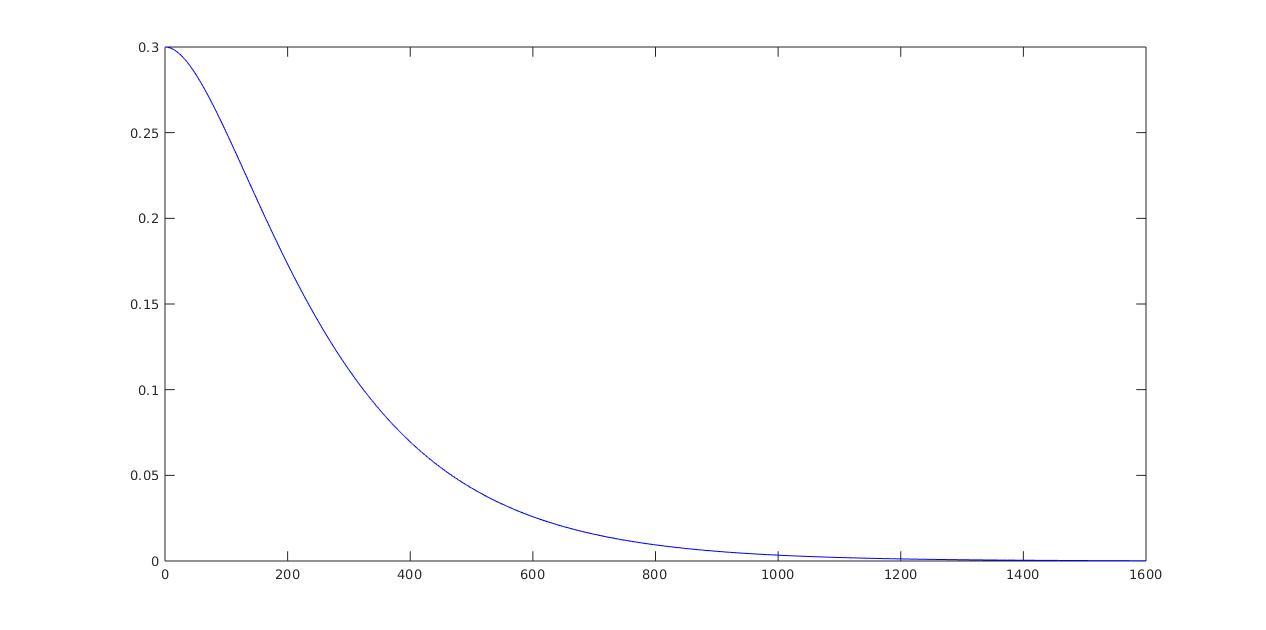
\includegraphics[width=0.8\textwidth]{inv_pen_Ku.jpg}
    \caption{Plotting Theta(t) based on $u=-Kx$}
    \label{fig:eig_inv_pendulum}
\end{figure}


\subsection{Segway - linear state space}

\lstinputlisting[firstline=1, lastline=20]{lin_space_rep_seg.m}

\subsection{Segway - controlablity}

\lstinputlisting[firstline=21, lastline=34]{lin_space_rep_seg.m}

\subsection{Segway - pole placement}

\lstinputlisting[firstline=35, lastline=131]{lin_space_rep_seg.m}

This was tested using 3 sets of pole placement values to get a good result. The initial placement has not been included in the plot as it did not converge.
the red line represents the $2^{nd}$ trial ($\lambda = [1,1,2,2]$) and the green represents the $3^{rd}$ ($\lambda = [1,2,3,4]$).

\begin{figure}[H]
    \centering
    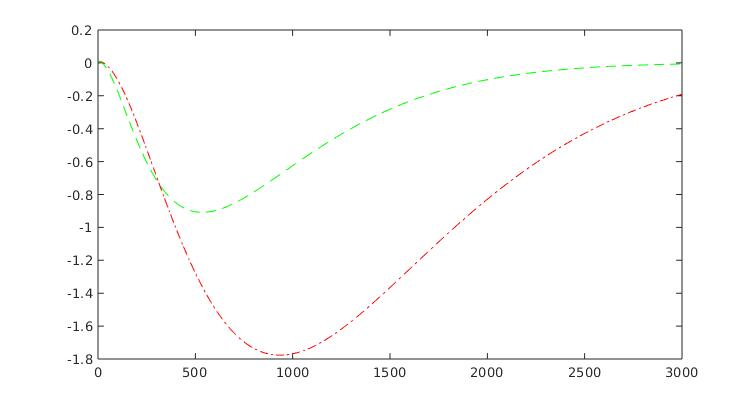
\includegraphics[width=0.6\textwidth]{x_pos_segway.jpg}
    \caption{Plotting x(t) based on $u=-Kx$}
    \label{fig:x_segway}
\end{figure}

\begin{figure}[H]
    \centering
    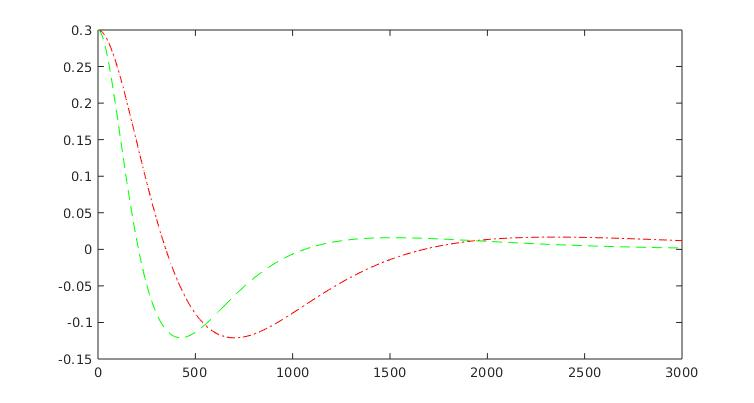
\includegraphics[width=0.6\textwidth]{th_pos_segway.jpg}
    \caption{Plotting Theta(t) based on $u=-Kx$}
    \label{fig:th_segway}
\end{figure}

\subsection{Segway - pole placement}

Using the best K from the previous section we determined that $x_0$ could be scaled by 3.33 and be able to converge.

\begin{figure}[H]
    \centering
    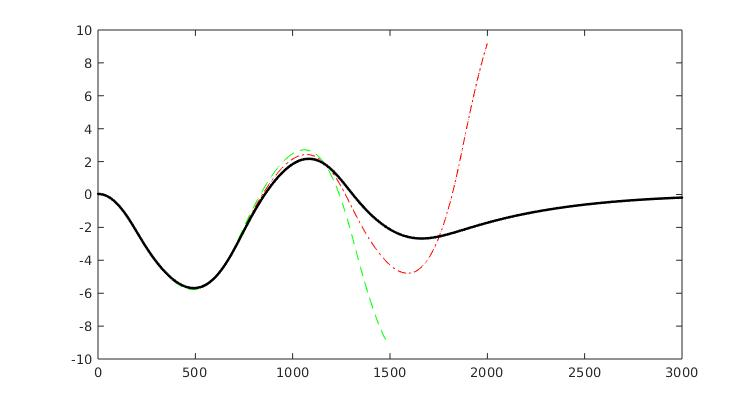
\includegraphics[width=0.6\textwidth]{x_t-max_scalar.jpg}
    \caption{x(t) based on scale values 3.35(green), 3.34(red), 3.33(black)}
    \label{fig:x_segway}
\end{figure}

\begin{figure}[H]
    \centering
    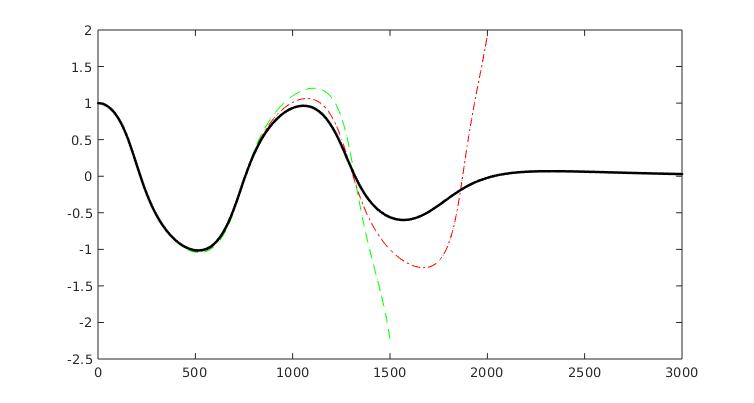
\includegraphics[width=0.6\textwidth]{th_t-max_scalar.jpg}
    \caption{Theta(t) based on scale values 3.35(green), 3.34(red), 3.33(black)}
    \label{fig:th_segway}
\end{figure}

\section{Observer Design}

\subsection{Observably}

\lstinputlisting[firstline=1, lastline=15]{observer.m}

\subsection{Observer Gain Matrix}

\lstinputlisting[firstline=17, lastline=56]{observer.m}

\subsection{Scaling}
\begin{figure}[H]
    \centering
    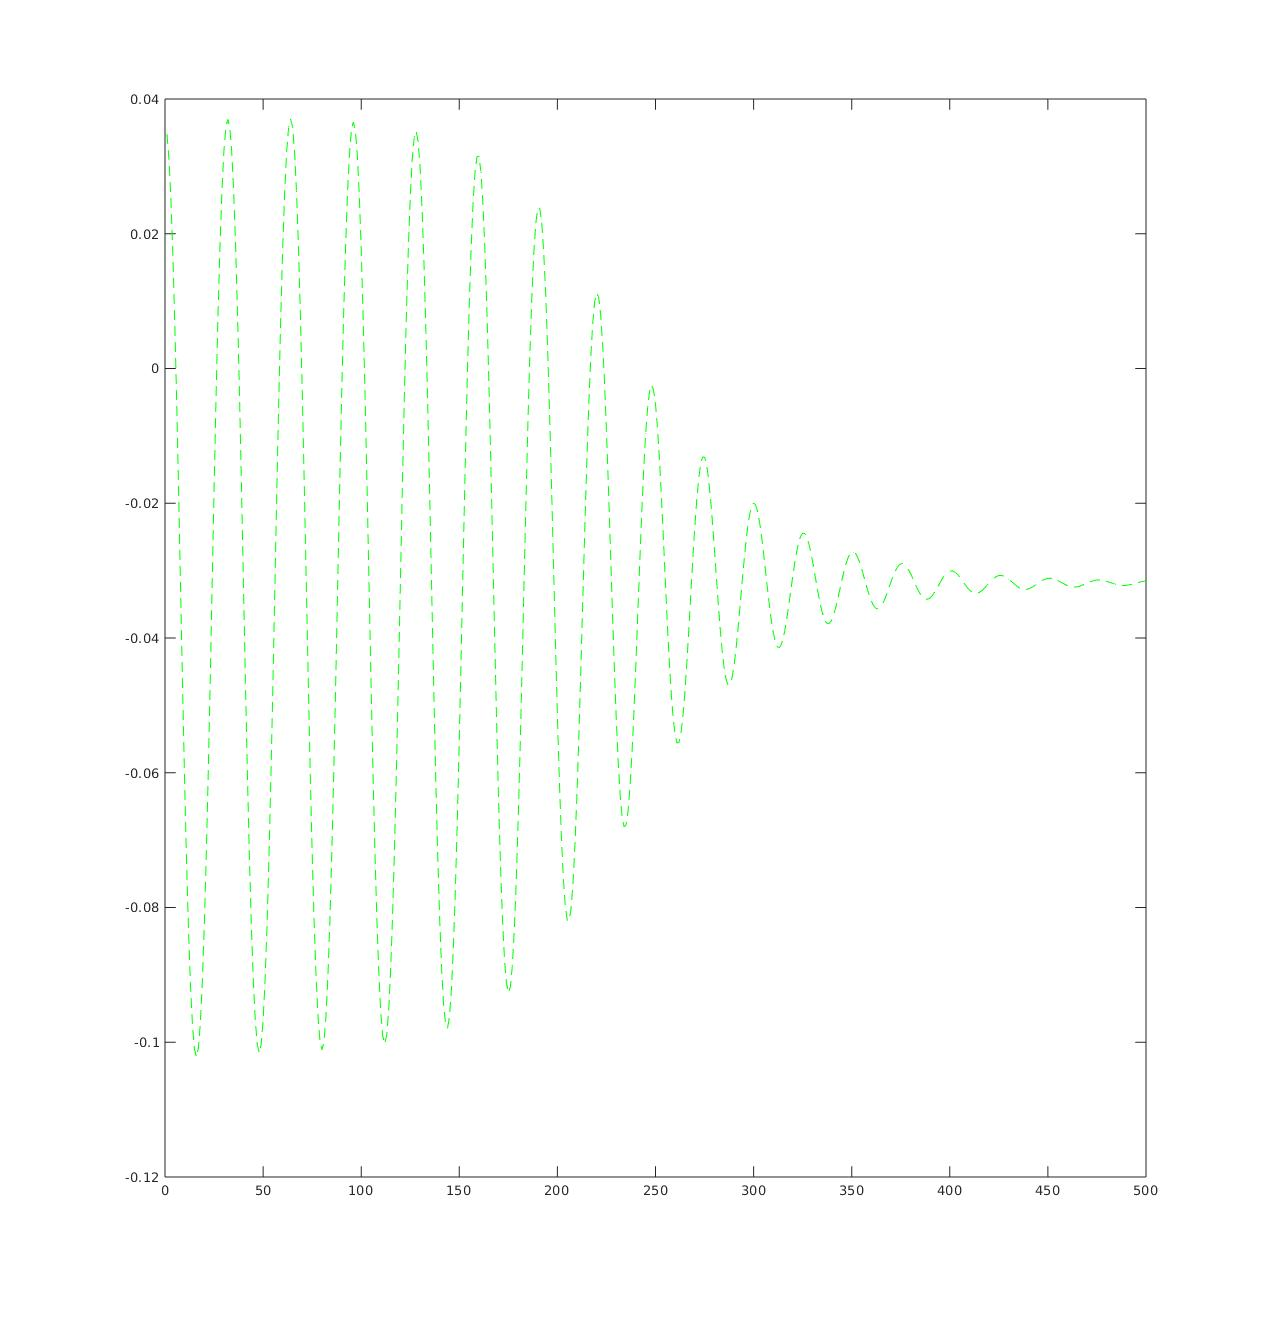
\includegraphics[width=0.6\textwidth]{x_pos_segway_obs.jpg}
    \caption{x(t) based on scale value 3.6}
    \label{fig:x_segway}
\end{figure}

\begin{figure}[H]
    \centering
    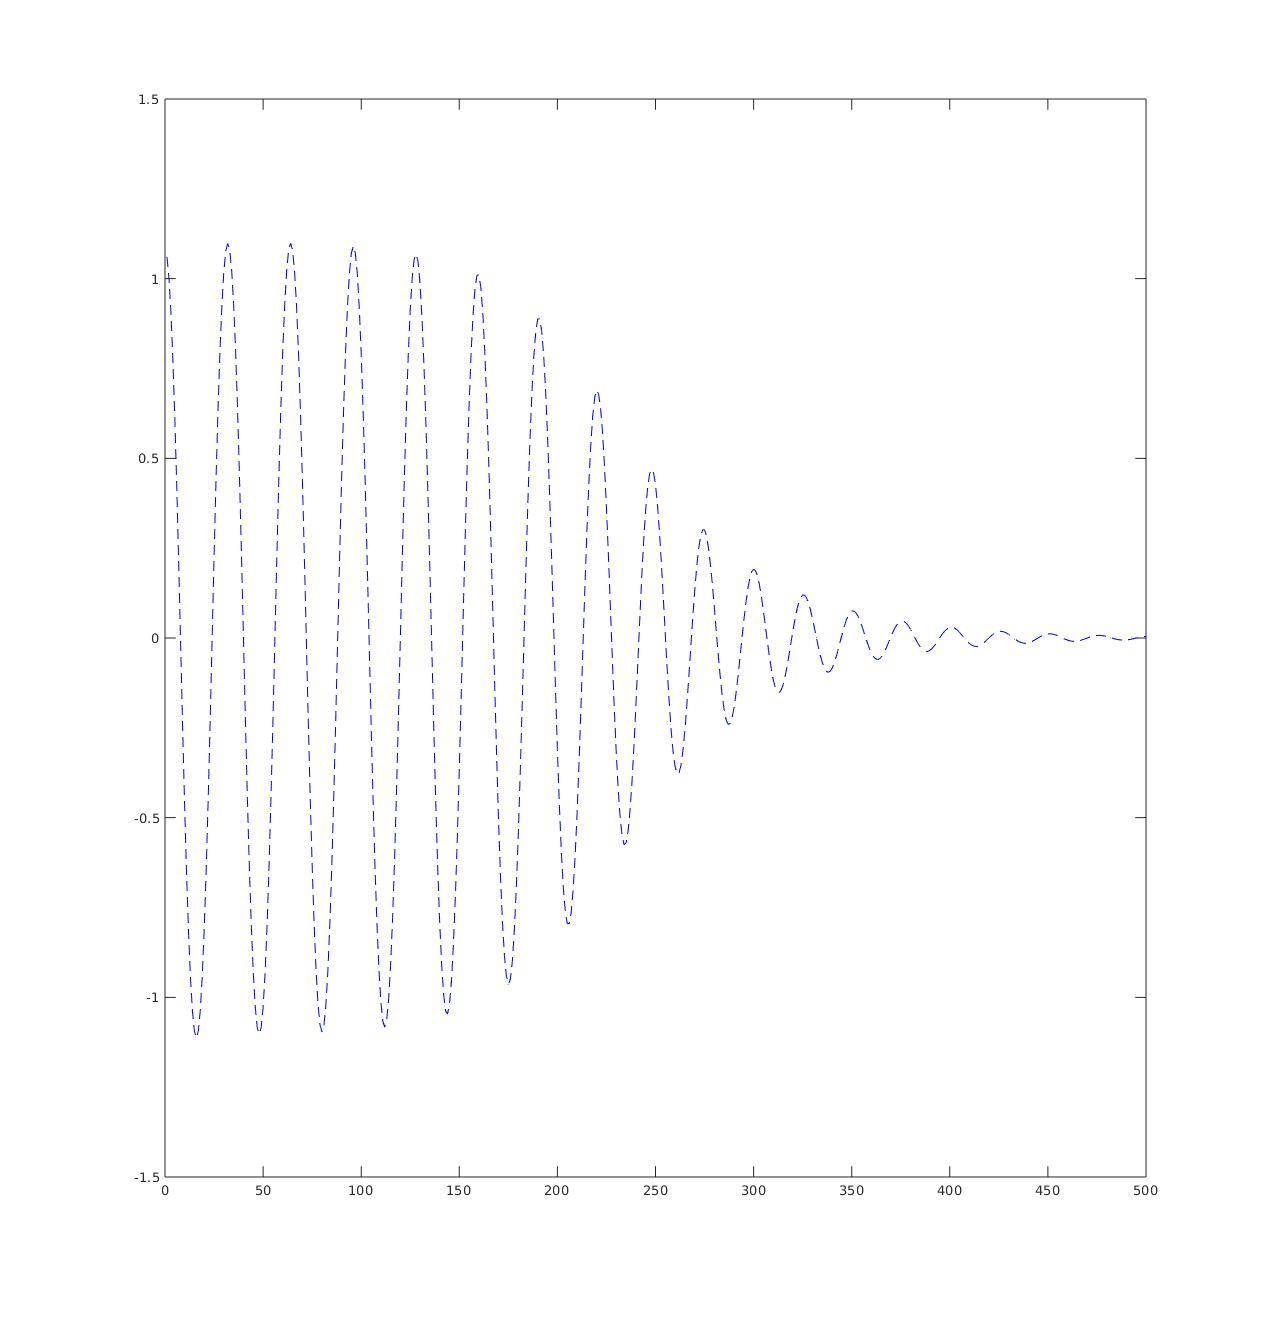
\includegraphics[width=0.6\textwidth]{th_pos_segway_obs.jpg}
    \caption{Theta(t) based on scale value 3.6}
    \label{fig:th_segway}
\end{figure}
Through testing we determined that the maximal scaling factor was about 3.6.

\subsection{Initial Scaling}
Setting only $\hat{x}_0$ to be scaled resulted in a much lower potential scaling factor of only about 2.6.

\begin{figure}[H]
    \centering
    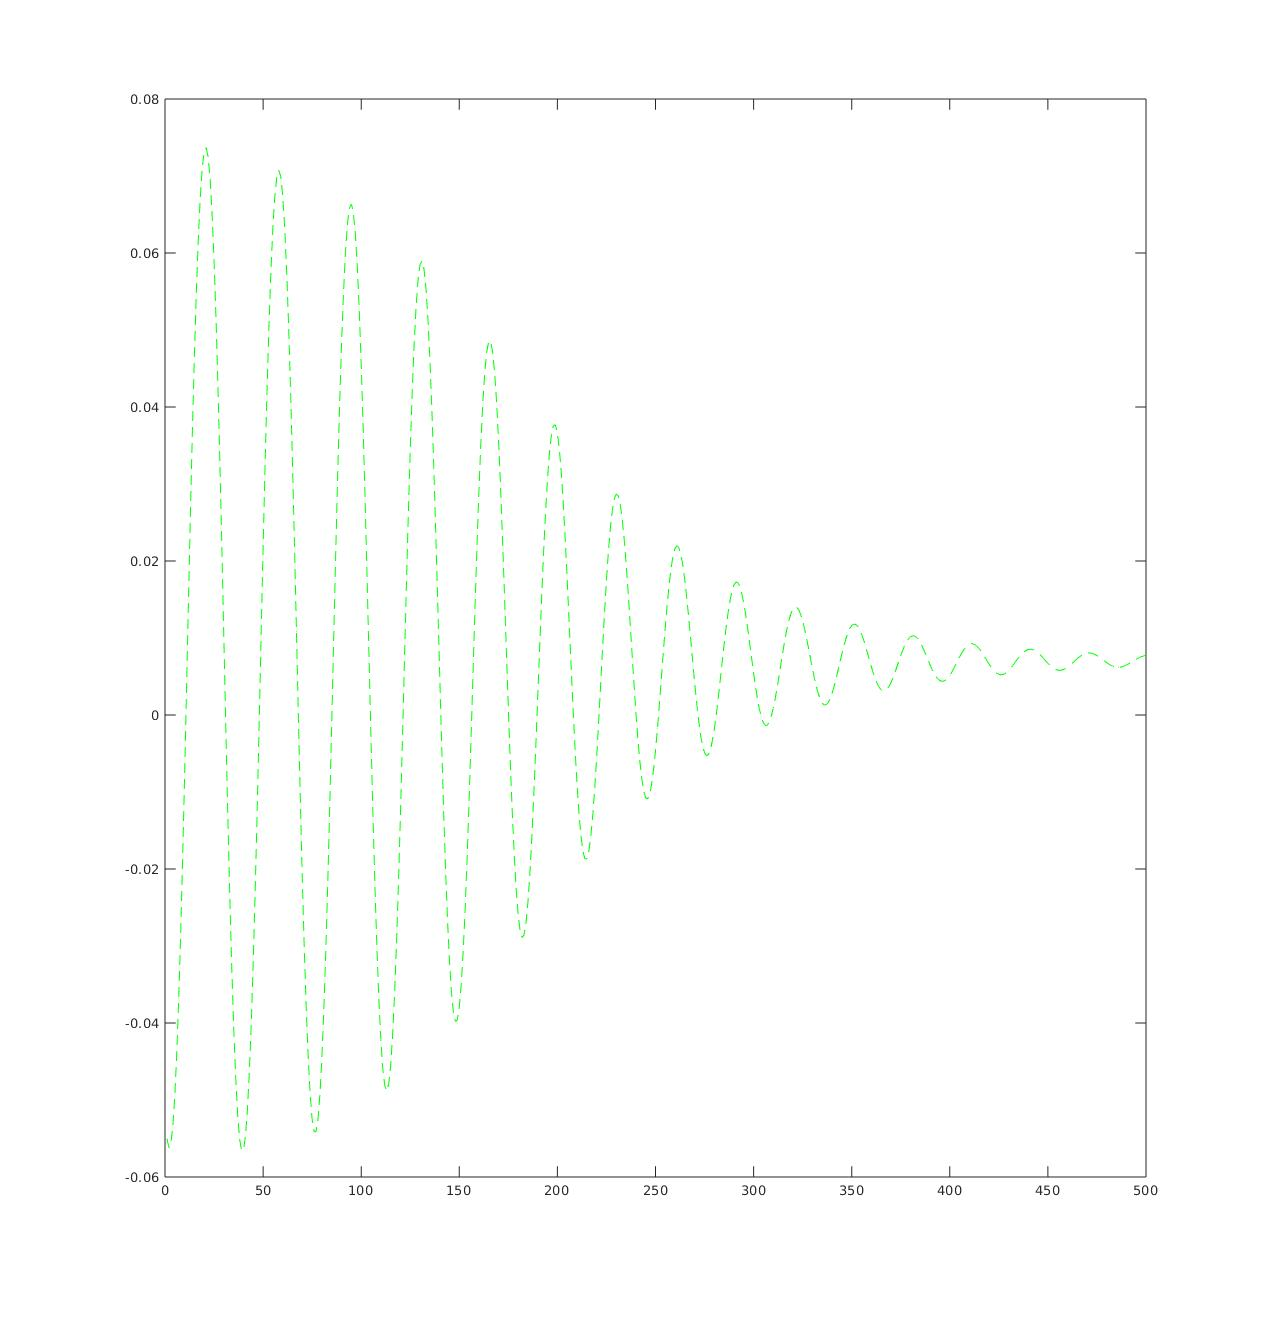
\includegraphics[width=0.6\textwidth]{x_pos_segway_obs_inital_only.jpg}
    \caption{x(t) based on scale value 2.6 of only $\hat{x}_0$}
    \label{fig:x_segway}
\end{figure}

\begin{figure}[H]
    \centering
    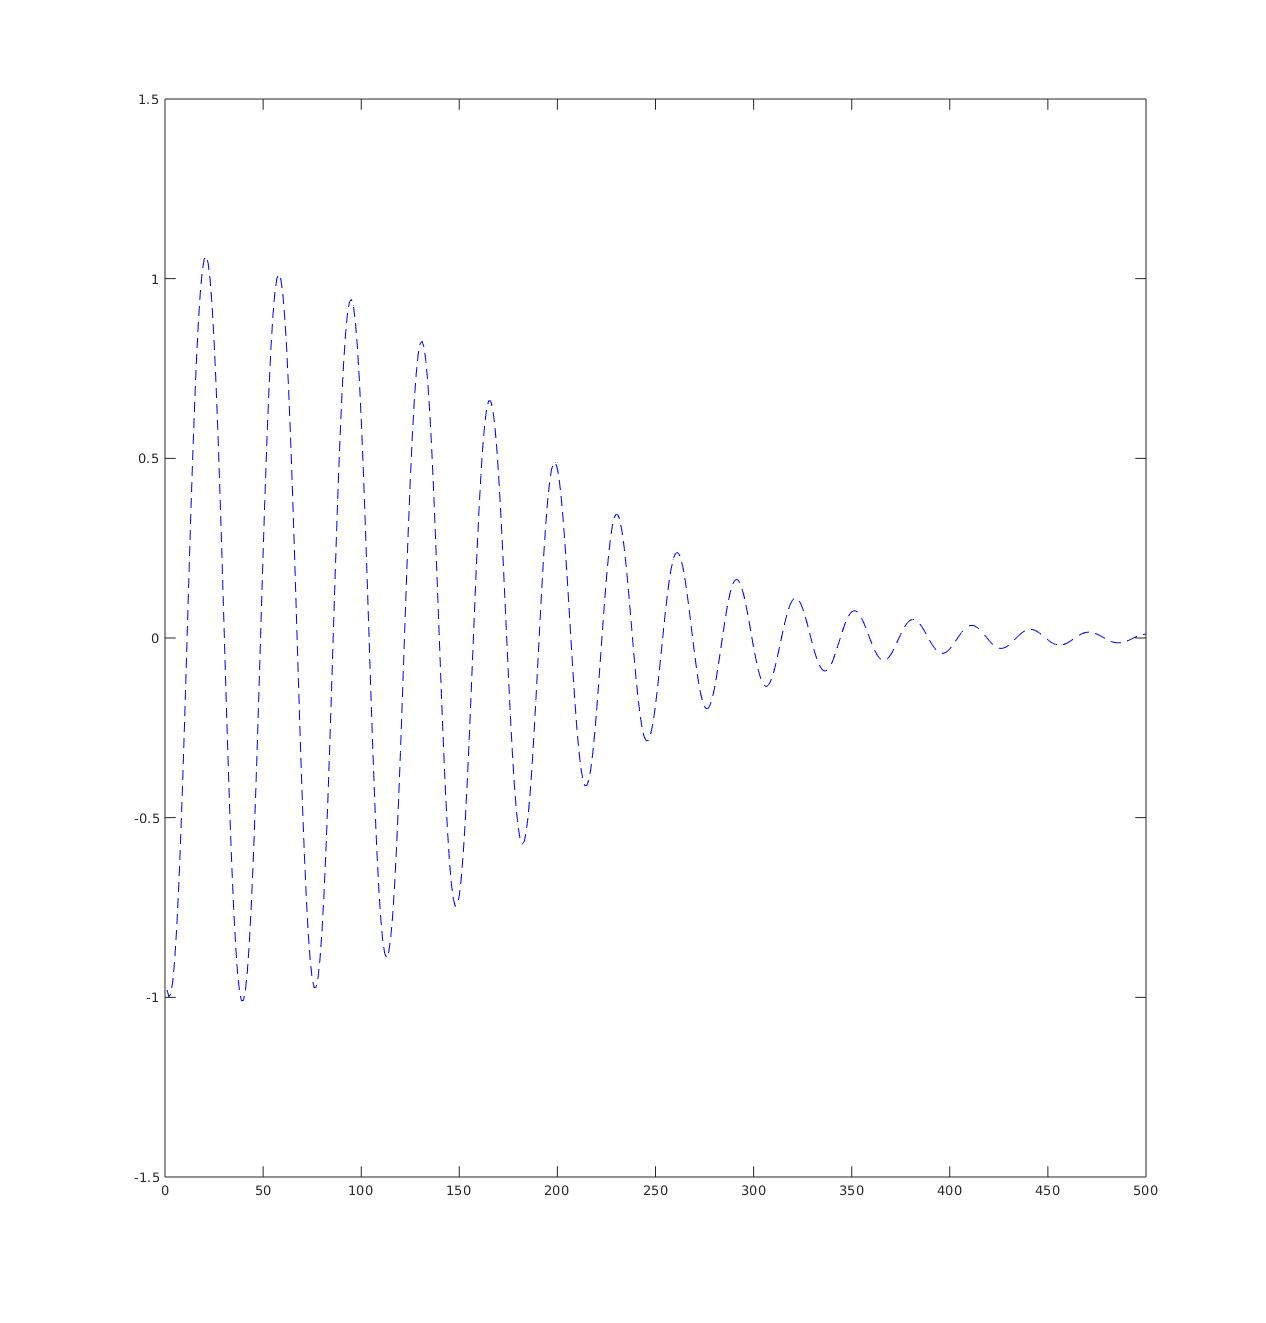
\includegraphics[width=0.6\textwidth]{th_pos_segway_obs_inital_only.jpg}
    \caption{Theta(t) based on scale value 2.6 of only $\hat{x}_0$}
    \label{fig:th_segway}
\end{figure}

\subsection{Tilt measurement}
By changing the C matrix I needed to change the P matrix to a value that would converge (-36 -36 1 1).

\begin{figure}[H]
    \centering
    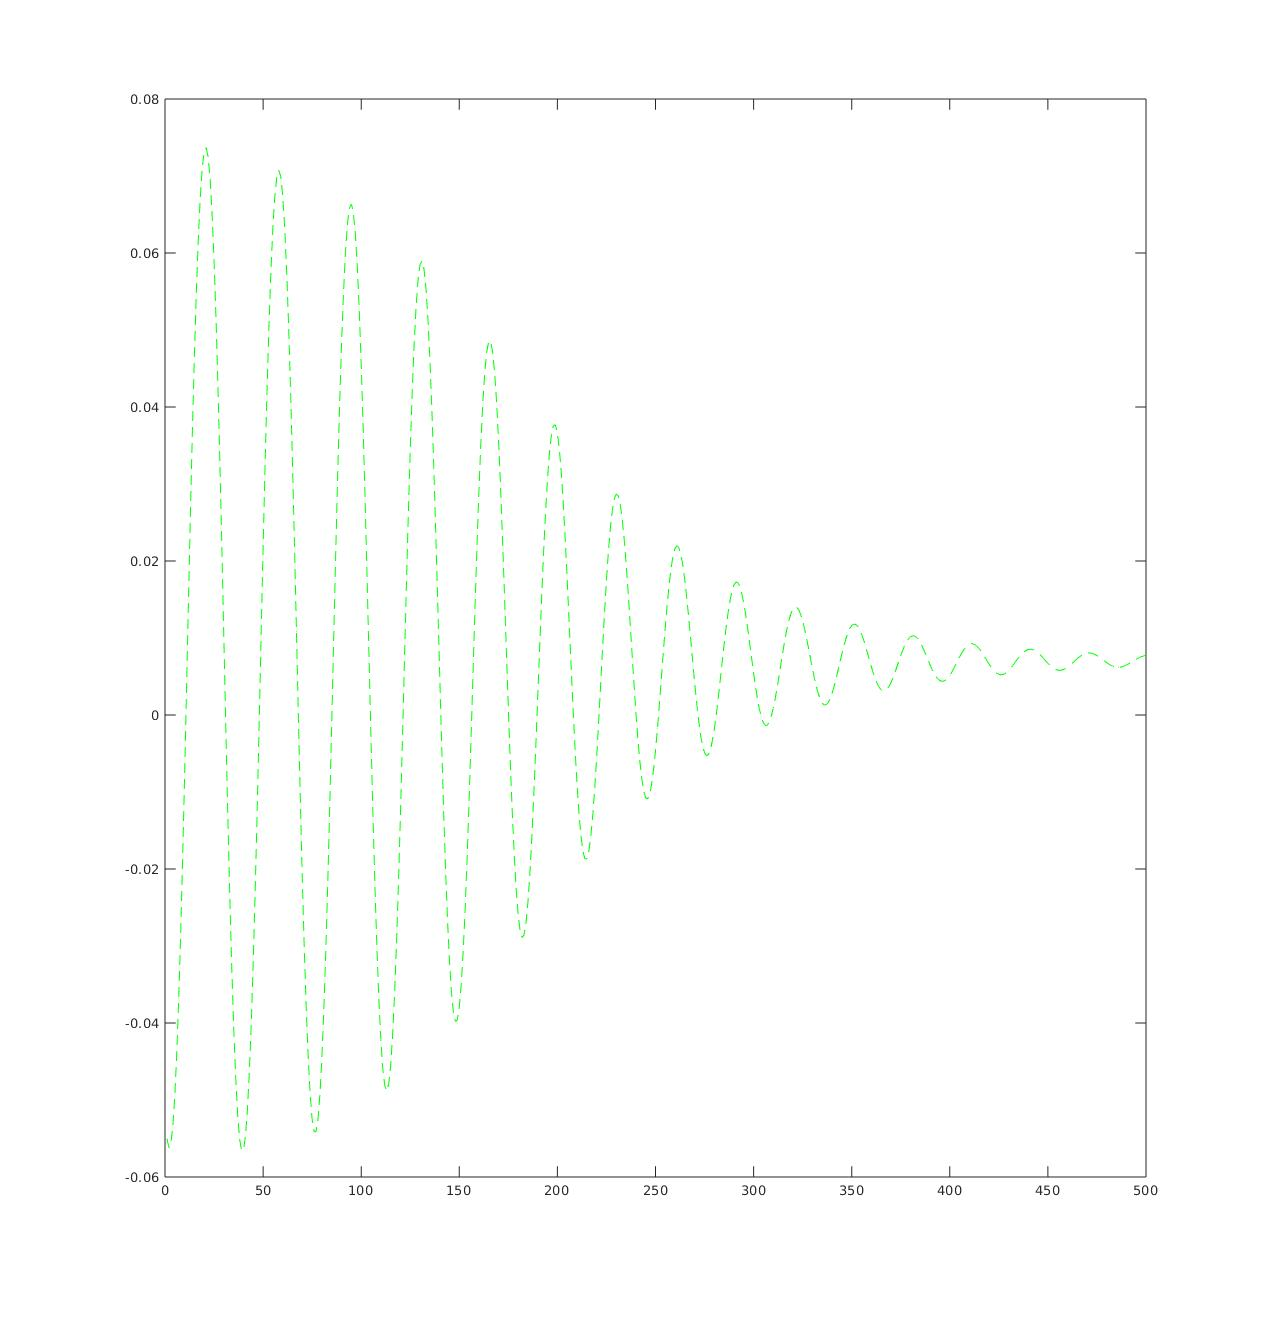
\includegraphics[width=0.6\textwidth]{x_pos_segway_obs_inital_only.jpg}
    \caption{x(t) with gyro as part of C matric}
    \label{fig:x_segway}
\end{figure}

\begin{figure}[H]
    \centering
    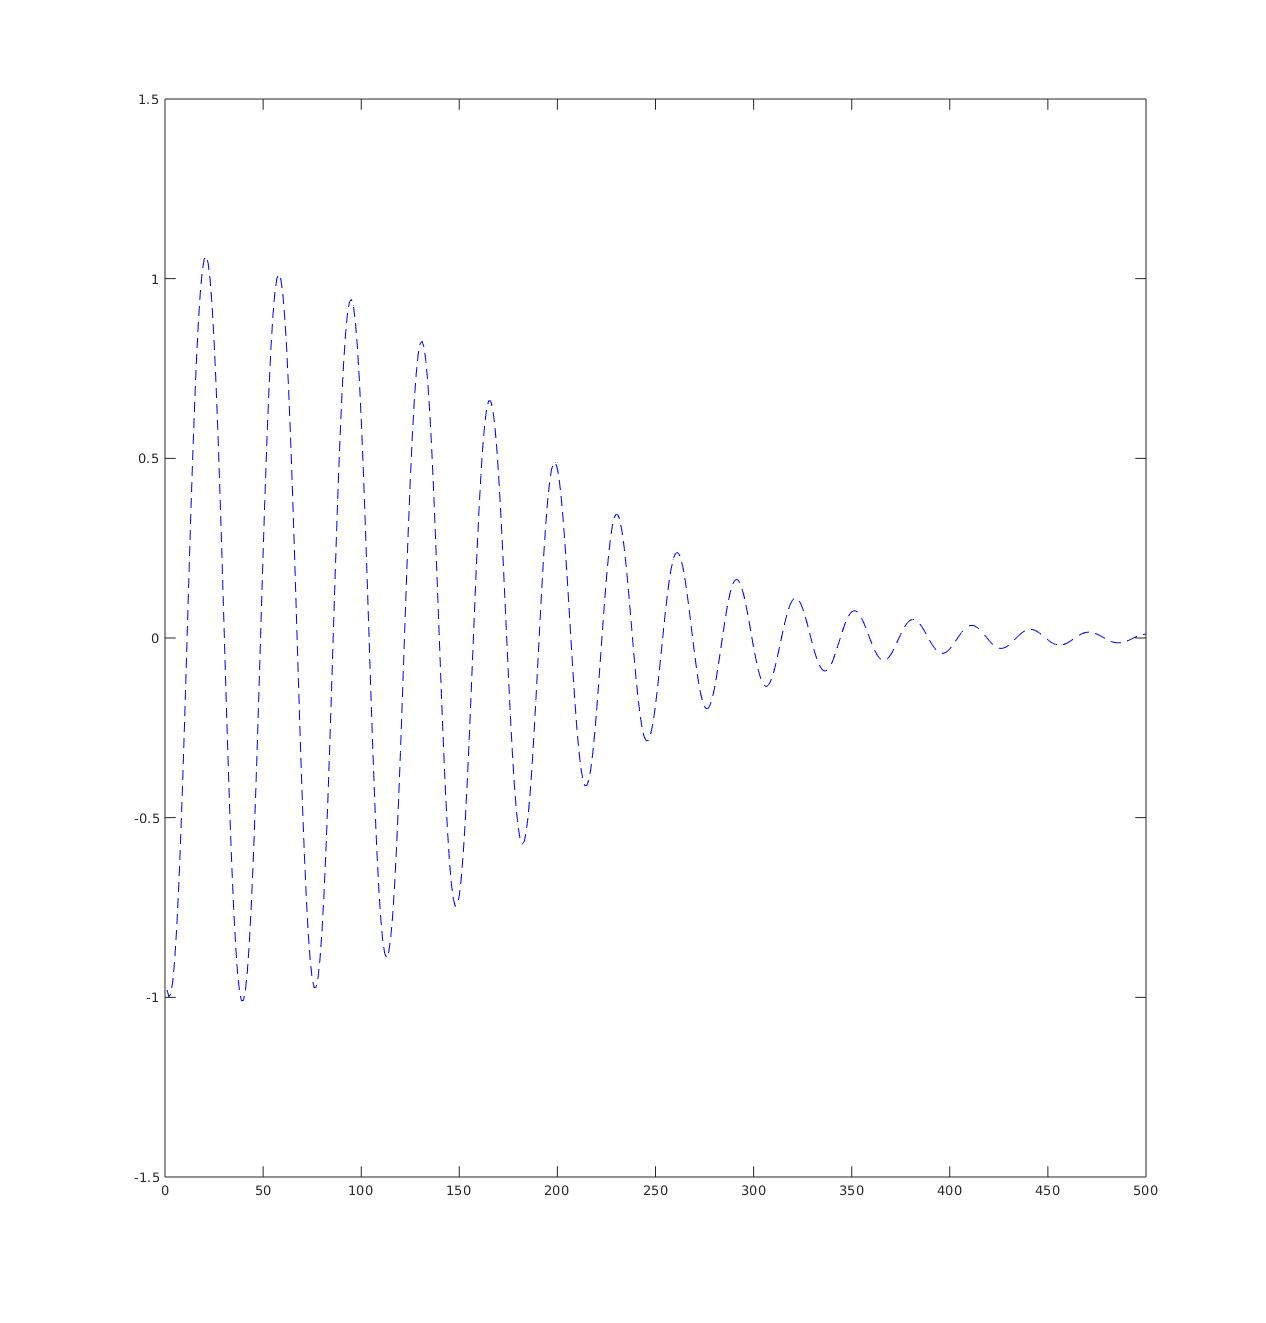
\includegraphics[width=0.6\textwidth]{th_pos_segway_obs_inital_only.jpg}
    \caption{Theta(t) with gyro as part of C matric}
    \label{fig:th_segway}
\end{figure}

I was able to get a higher scaling factor for a global initial scale in this situation.
\begin{figure}[H]
    \centering
    \includegraphics[width=0.8\textwidth]{seg_giro_4_3.jpg}
    \caption{x(t) with gyro as part of C matric scaled by 4.33}
\end{figure}

\begin{figure}[H]
    \centering
    \includegraphics[width=0.8\textwidth]{seg_giro_4_3_th.jpg}
    \caption{Theta(t) with gyro as part of C matric scaled by 4.33}
    \label{fig:th_segway}
\end{figure}

Setting only $\hat{x}_0$ to be scaled resulted in a much lower potential scaling factor of only about 2.6.
\begin{figure}[H]
    \centering
    \includegraphics[width=0.6\textwidth]{xpos_segway_obs_inital_only_1_25.jpg}
    \caption{x(t) with gyro as part of C matric scaled by 1.25 of only for $\hat{x}_0$}
    \label{fig:x_segway}
\end{figure}

\begin{figure}[H]
    \centering
    \includegraphics[width=0.6\textwidth]{thpos_segway_obs_inital_only_1_25.jpg}
    \caption{Theta(t) with gyro as part of C matric scaled by 1.25 of only for $\hat{x}_0$}
    \label{fig:th_segway}
\end{figure}

Setting only $\hat{x}_0$ to be scaled resulted in a much much lower potential scaling factor of only about 1.25.

\subsection{Reference Gain}
\begin{figure}[H]
    \centering
    \includegraphics[width=0.8\textwidth]{seg_giro_4_3.jpg}
    \caption{x(t) with gain matrix -- r(t) = 1}
    \label{fig:x_segway}
\end{figure}

\begin{figure}[H]
    \centering
    \includegraphics[width=0.8\textwidth]{seg_giro_4_3_th.jpg}
    \caption{Theta(t) with gain matrix -- r(t) = sin(t)}
    \label{fig:th_segway}
\end{figure}

\section{Code}
    \texttt{inv\_pend\_test.m} - inverse pendulum test with u calculated with pid or -Kx

    \texttt{segway\_test.m} - segway with control calculated u, with tests for max scaled initial state

    \texttt{segway\_gains.m} - segway with gain matrix added

    \texttt{segway\_giro\_test.m} - segway with giro controller added in

    \texttt{segway\_obs\_test.m} - test function for segway using observer calculations

    \texttt{segway\_test\_initial\_state.m} - segway test script for initial scaling using the control function

    \texttt{observer.m} - calculations for observably

    \texttt{lin\_space\_rep\_seg.m} - calculations for segway control

    \texttt{lin\_space\_test.m} - test for inverse pendulum control

    \texttt{lin\_space\_rep.m} - calculations for inverse pendulum control

    \texttt{PIDController} - pid class for inverse pendulum

\end{document}
